\documentclass{standalone}
\usepackage{tikz}
\usetikzlibrary{patterns}
\usetikzlibrary{positioning}
\usetikzlibrary{patterns, positioning}
\usetikzlibrary{shapes.misc}
\usepackage[outline]{contour}
\contourlength{1.5pt} 
\usetikzlibrary{calc}
        \usepackage{relsize}
        \tikzset{fontscale/.style = {font=\relsize{#1}}}

\begin{document}
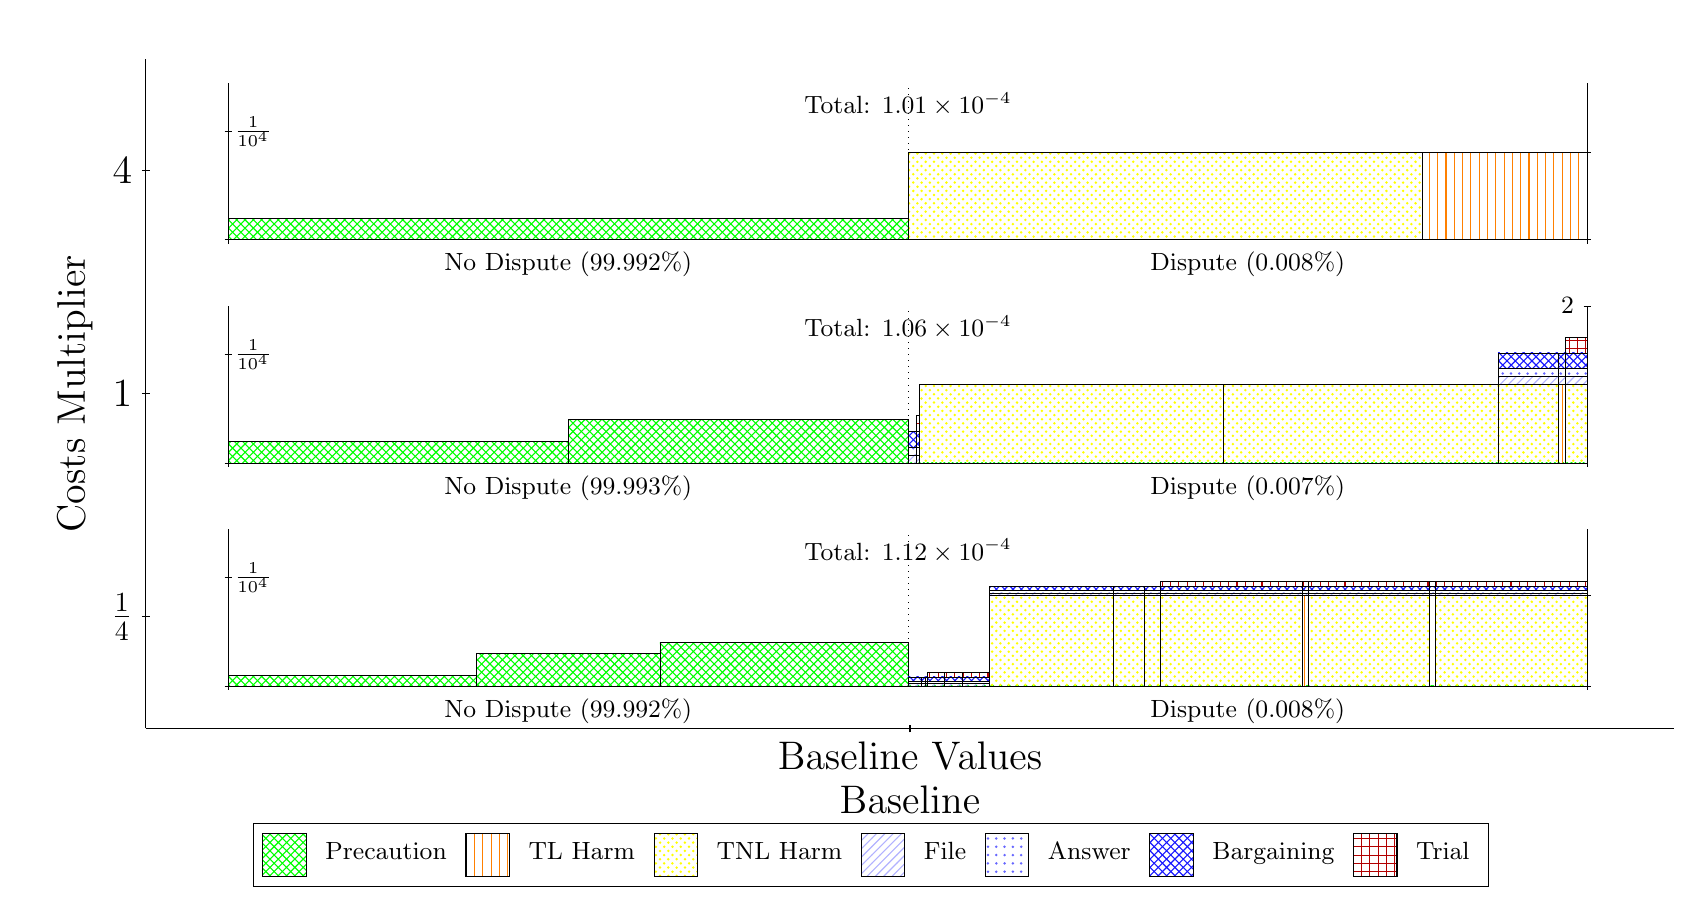
\begin{tikzpicture}
\clip(-0.5,-1.1) rectangle +(20.91,11);
\draw[black] (1,1) -- (1,9.5);
\node[rotate=90, fontscale=2, anchor=center] at (0.1, 5.25) {Costs Multiplier};
\draw[black] (0.95,2.4167) -- (1.05,2.4167);
\node[fontscale=2, anchor=east] at (0.95, 2.4167) {$\frac{1}{4}$};
\draw[black] (0.95,5.25) -- (1.05,5.25);
\node[fontscale=2, anchor=east] at (0.95, 5.25) {1};
\draw[black] (0.95,8.0833) -- (1.05,8.0833);
\node[fontscale=2, anchor=east] at (0.95, 8.0833) {4};

\draw[black] (1,1) -- (20.41,1);
\node[fontscale=2, anchor=center] at (10.705, 0.1) {Baseline};
\draw[black] (10.705,0.95) -- (10.705,1.05);
\node[fontscale=2, anchor=north] at (10.705, 0.95) {Baseline Values};


\draw[pattern=crosshatch, pattern color=green,draw=black,very thin] (2.05,1.54) rectangle (5.201,1.6774);
\draw[pattern=crosshatch, pattern color=green,draw=black,very thin] (5.201,1.54) rectangle (7.5289,1.9522);
\draw[pattern=crosshatch, pattern color=green,draw=black,very thin] (7.5289,1.54) rectangle (10.68,2.0896);
\draw[pattern=crosshatch, pattern color=green,draw=black,very thin] (10.68,1.54) rectangle (10.851,1.54);
\draw[pattern=north east lines, pattern color=blue!30,draw=black,very thin] (10.68,1.54) rectangle (10.851,1.5688);
\draw[pattern=dots,  pattern color=blue!60,draw=black,very thin] (10.68,1.5688) rectangle (10.851,1.5977);
\draw[pattern=crosshatch,      pattern color=blue!90,draw=black,very thin] (10.68,1.5977) rectangle (10.851,1.6553);
\draw[pattern=crosshatch, pattern color=green,draw=black,very thin] (10.851,1.54) rectangle (10.901,1.54);
\draw[pattern=north east lines, pattern color=blue!30,draw=black,very thin] (10.851,1.54) rectangle (10.901,1.5689);
\draw[pattern=dots,  pattern color=blue!60,draw=black,very thin] (10.851,1.5689) rectangle (10.901,1.5977);
\draw[pattern=crosshatch,      pattern color=blue!90,draw=black,very thin] (10.851,1.5977) rectangle (10.901,1.6553);
\draw[pattern=crosshatch, pattern color=green,draw=black,very thin] (10.901,1.54) rectangle (10.931,1.54);
\draw[pattern=north east lines, pattern color=blue!30,draw=black,very thin] (10.901,1.54) rectangle (10.931,1.5689);
\draw[pattern=dots,  pattern color=blue!60,draw=black,very thin] (10.901,1.5689) rectangle (10.931,1.5977);
\draw[pattern=crosshatch,      pattern color=blue!90,draw=black,very thin] (10.901,1.5977) rectangle (10.931,1.6553);
\draw[pattern=crosshatch, pattern color=green,draw=black,very thin] (10.931,1.54) rectangle (11.136,1.54);
\draw[pattern=north east lines, pattern color=blue!30,draw=black,very thin] (10.931,1.54) rectangle (11.136,1.5688);
\draw[pattern=dots,  pattern color=blue!60,draw=black,very thin] (10.931,1.5688) rectangle (11.136,1.5977);
\draw[pattern=crosshatch,      pattern color=blue!90,draw=black,very thin] (10.931,1.5977) rectangle (11.136,1.6553);
\draw[pattern=grid,            pattern color=red!70!black,draw=black,very thin] (10.931,1.6553) rectangle (11.136,1.713);
\draw[pattern=crosshatch, pattern color=green,draw=black,very thin] (11.136,1.54) rectangle (11.363,1.54);
\draw[pattern=north east lines, pattern color=blue!30,draw=black,very thin] (11.136,1.54) rectangle (11.363,1.5689);
\draw[pattern=dots,  pattern color=blue!60,draw=black,very thin] (11.136,1.5689) rectangle (11.363,1.5977);
\draw[pattern=crosshatch,      pattern color=blue!90,draw=black,very thin] (11.136,1.5977) rectangle (11.363,1.6553);
\draw[pattern=grid,            pattern color=red!70!black,draw=black,very thin] (11.136,1.6553) rectangle (11.363,1.713);
\draw[pattern=crosshatch, pattern color=green,draw=black,very thin] (11.363,1.54) rectangle (11.71,1.54);
\draw[pattern=north east lines, pattern color=blue!30,draw=black,very thin] (11.363,1.54) rectangle (11.71,1.5689);
\draw[pattern=dots,  pattern color=blue!60,draw=black,very thin] (11.363,1.5689) rectangle (11.71,1.5977);
\draw[pattern=crosshatch,      pattern color=blue!90,draw=black,very thin] (11.363,1.5977) rectangle (11.71,1.6553);
\draw[pattern=grid,            pattern color=red!70!black,draw=black,very thin] (11.363,1.6553) rectangle (11.71,1.713);
\draw[pattern=crosshatch, pattern color=green,draw=black,very thin] (11.71,1.54) rectangle (13.288,1.54);
\draw[pattern=crosshatch dots, pattern color=yellow,draw=black,very thin] (11.71,1.54) rectangle (13.288,2.693);
\draw[pattern=north east lines, pattern color=blue!30,draw=black,very thin] (11.71,2.693) rectangle (13.288,2.7218);
\draw[pattern=dots,  pattern color=blue!60,draw=black,very thin] (11.71,2.7218) rectangle (13.288,2.7507);
\draw[pattern=crosshatch,      pattern color=blue!90,draw=black,very thin] (11.71,2.7507) rectangle (13.288,2.8083);
\draw[pattern=crosshatch, pattern color=green,draw=black,very thin] (13.288,1.54) rectangle (13.29,1.54);
\draw[pattern=vertical lines, pattern color=orange,draw=black,very thin] (13.288,1.54) rectangle (13.29,2.693);
\draw[pattern=north east lines, pattern color=blue!30,draw=black,very thin] (13.288,2.693) rectangle (13.29,2.7218);
\draw[pattern=dots,  pattern color=blue!60,draw=black,very thin] (13.288,2.7218) rectangle (13.29,2.7507);
\draw[pattern=crosshatch,      pattern color=blue!90,draw=black,very thin] (13.288,2.7507) rectangle (13.29,2.8083);
\draw[pattern=crosshatch, pattern color=green,draw=black,very thin] (13.29,1.54) rectangle (13.682,1.54);
\draw[pattern=crosshatch dots, pattern color=yellow,draw=black,very thin] (13.29,1.54) rectangle (13.682,2.693);
\draw[pattern=north east lines, pattern color=blue!30,draw=black,very thin] (13.29,2.693) rectangle (13.682,2.7219);
\draw[pattern=dots,  pattern color=blue!60,draw=black,very thin] (13.29,2.7219) rectangle (13.682,2.7507);
\draw[pattern=crosshatch,      pattern color=blue!90,draw=black,very thin] (13.29,2.7507) rectangle (13.682,2.8083);
\draw[pattern=crosshatch, pattern color=green,draw=black,very thin] (13.682,1.54) rectangle (13.881,1.54);
\draw[pattern=crosshatch dots, pattern color=yellow,draw=black,very thin] (13.682,1.54) rectangle (13.881,2.693);
\draw[pattern=north east lines, pattern color=blue!30,draw=black,very thin] (13.682,2.693) rectangle (13.881,2.7219);
\draw[pattern=dots,  pattern color=blue!60,draw=black,very thin] (13.682,2.7219) rectangle (13.881,2.7507);
\draw[pattern=crosshatch,      pattern color=blue!90,draw=black,very thin] (13.682,2.7507) rectangle (13.881,2.8083);
\draw[pattern=crosshatch, pattern color=green,draw=black,very thin] (13.881,1.54) rectangle (15.681,1.54);
\draw[pattern=crosshatch dots, pattern color=yellow,draw=black,very thin] (13.881,1.54) rectangle (15.681,2.693);
\draw[pattern=north east lines, pattern color=blue!30,draw=black,very thin] (13.881,2.693) rectangle (15.681,2.7218);
\draw[pattern=dots,  pattern color=blue!60,draw=black,very thin] (13.881,2.7218) rectangle (15.681,2.7507);
\draw[pattern=crosshatch,      pattern color=blue!90,draw=black,very thin] (13.881,2.7507) rectangle (15.681,2.8083);
\draw[pattern=grid,            pattern color=red!70!black,draw=black,very thin] (13.881,2.8083) rectangle (15.681,2.866);
\draw[pattern=crosshatch, pattern color=green,draw=black,very thin] (15.681,1.54) rectangle (15.759,1.54);
\draw[pattern=vertical lines, pattern color=orange,draw=black,very thin] (15.681,1.54) rectangle (15.759,2.693);
\draw[pattern=north east lines, pattern color=blue!30,draw=black,very thin] (15.681,2.693) rectangle (15.759,2.7218);
\draw[pattern=dots,  pattern color=blue!60,draw=black,very thin] (15.681,2.7218) rectangle (15.759,2.7507);
\draw[pattern=crosshatch,      pattern color=blue!90,draw=black,very thin] (15.681,2.7507) rectangle (15.759,2.8083);
\draw[pattern=grid,            pattern color=red!70!black,draw=black,very thin] (15.681,2.8083) rectangle (15.759,2.866);
\draw[pattern=crosshatch, pattern color=green,draw=black,very thin] (15.759,1.54) rectangle (17.295,1.54);
\draw[pattern=crosshatch dots, pattern color=yellow,draw=black,very thin] (15.759,1.54) rectangle (17.295,2.693);
\draw[pattern=north east lines, pattern color=blue!30,draw=black,very thin] (15.759,2.693) rectangle (17.295,2.7219);
\draw[pattern=dots,  pattern color=blue!60,draw=black,very thin] (15.759,2.7219) rectangle (17.295,2.7507);
\draw[pattern=crosshatch,      pattern color=blue!90,draw=black,very thin] (15.759,2.7507) rectangle (17.295,2.8083);
\draw[pattern=grid,            pattern color=red!70!black,draw=black,very thin] (15.759,2.8083) rectangle (17.295,2.866);
\draw[pattern=crosshatch, pattern color=green,draw=black,very thin] (17.295,1.54) rectangle (17.371,1.54);
\draw[pattern=vertical lines, pattern color=orange,draw=black,very thin] (17.295,1.54) rectangle (17.371,2.693);
\draw[pattern=north east lines, pattern color=blue!30,draw=black,very thin] (17.295,2.693) rectangle (17.371,2.7219);
\draw[pattern=dots,  pattern color=blue!60,draw=black,very thin] (17.295,2.7219) rectangle (17.371,2.7507);
\draw[pattern=crosshatch,      pattern color=blue!90,draw=black,very thin] (17.295,2.7507) rectangle (17.371,2.8083);
\draw[pattern=grid,            pattern color=red!70!black,draw=black,very thin] (17.295,2.8083) rectangle (17.371,2.866);
\draw[pattern=crosshatch, pattern color=green,draw=black,very thin] (17.371,1.54) rectangle (19.31,1.54);
\draw[pattern=crosshatch dots, pattern color=yellow,draw=black,very thin] (17.371,1.54) rectangle (19.31,2.693);
\draw[pattern=north east lines, pattern color=blue!30,draw=black,very thin] (17.371,2.693) rectangle (19.31,2.7219);
\draw[pattern=dots,  pattern color=blue!60,draw=black,very thin] (17.371,2.7219) rectangle (19.31,2.7507);
\draw[pattern=crosshatch,      pattern color=blue!90,draw=black,very thin] (17.371,2.7507) rectangle (19.31,2.8083);
\draw[pattern=grid,            pattern color=red!70!black,draw=black,very thin] (17.371,2.8083) rectangle (19.31,2.866);
\node[font=\small,text=black,anchor=north] at (10.68, 3.5333) {Total: $1.12\times 10^{-4}$};
\draw[black,very thin] (2.05,1.54) -- (2.05,3.5333);
\draw[black,very thin] (2,1.54) -- (2.1,1.54);
\node[font=\small,text=black, anchor=west] at (2, 1.54) {};
\draw[black,very thin] (2,2.914) -- (2.1,2.914);
\node[font=\small,text=black, anchor=west] at (2, 2.914) {$\frac{1}{10^{4}}$};

\draw[black,dotted,very thin] (10.68,1.5998) -- (10.68,3.4735);
\draw[black,very thin] (19.31,1.54) -- (19.31,3.5333);
\draw[black,very thin] (19.26,1.54) -- (19.36,1.54);
\node[font=\small,text=black, anchor=east] at (19.26, 1.54) {\contour{white}{}};
\draw[black,very thin] (19.26,2.693) -- (19.36,2.693);
\node[font=\small,text=black, anchor=east] at (19.26, 2.693) {\contour{white}{}};

\draw[black,very thin] (2.05,1.54) -- (19.31,1.54);
\draw[black,very thin] (2.05,1.49) -- (2.05,1.59);
\node[font=\small,text=black, anchor=north] at (2.05, 1.49) {};
\draw[black,very thin] (19.31,1.49) -- (19.31,1.59);
\node[font=\small,text=black, anchor=north] at (19.31, 1.49) {};

\node[font=\small,text=black,anchor=south] at (6.365, 0.94) {No\ Dispute\ (99.992\%)};
\node[font=\small,text=black,anchor=south] at (14.995, 0.94) {Dispute\ (0.008\%)};

\draw[pattern=crosshatch, pattern color=green,draw=black,very thin] (2.05,4.3733) rectangle (6.3649,4.6481);
\draw[pattern=crosshatch, pattern color=green,draw=black,very thin] (6.3649,4.3733) rectangle (10.68,4.9229);
\draw[pattern=crosshatch, pattern color=green,draw=black,very thin] (10.68,4.3733) rectangle (10.787,4.3734);
\draw[pattern=north east lines, pattern color=blue!30,draw=black,very thin] (10.68,4.3734) rectangle (10.787,4.473);
\draw[pattern=dots,  pattern color=blue!60,draw=black,very thin] (10.68,4.473) rectangle (10.787,4.5727);
\draw[pattern=crosshatch,      pattern color=blue!90,draw=black,very thin] (10.68,4.5727) rectangle (10.787,4.772);
\draw[pattern=crosshatch, pattern color=green,draw=black,very thin] (10.787,4.3733) rectangle (10.821,4.3734);
\draw[pattern=north east lines, pattern color=blue!30,draw=black,very thin] (10.787,4.3734) rectangle (10.821,4.473);
\draw[pattern=dots,  pattern color=blue!60,draw=black,very thin] (10.787,4.473) rectangle (10.821,4.5727);
\draw[pattern=crosshatch,      pattern color=blue!90,draw=black,very thin] (10.787,4.5727) rectangle (10.821,4.772);
\draw[pattern=grid,            pattern color=red!70!black,draw=black,very thin] (10.787,4.772) rectangle (10.821,4.9713);
\draw[pattern=crosshatch, pattern color=green,draw=black,very thin] (10.821,4.3733) rectangle (14.686,4.3734);
\draw[pattern=crosshatch dots, pattern color=yellow,draw=black,very thin] (10.821,4.3734) rectangle (14.686,5.37);
\draw[pattern=crosshatch, pattern color=green,draw=black,very thin] (14.686,4.3733) rectangle (14.689,4.3734);
\draw[pattern=vertical lines, pattern color=orange,draw=black,very thin] (14.686,4.3734) rectangle (14.689,5.37);
\draw[pattern=crosshatch, pattern color=green,draw=black,very thin] (14.689,4.3733) rectangle (18.173,4.3734);
\draw[pattern=crosshatch dots, pattern color=yellow,draw=black,very thin] (14.689,4.3734) rectangle (18.173,5.37);
\draw[pattern=crosshatch, pattern color=green,draw=black,very thin] (18.173,4.3733) rectangle (18.933,4.3734);
\draw[pattern=crosshatch dots, pattern color=yellow,draw=black,very thin] (18.173,4.3734) rectangle (18.933,5.37);
\draw[pattern=north east lines, pattern color=blue!30,draw=black,very thin] (18.173,5.37) rectangle (18.933,5.4697);
\draw[pattern=dots,  pattern color=blue!60,draw=black,very thin] (18.173,5.4697) rectangle (18.933,5.5693);
\draw[pattern=crosshatch,      pattern color=blue!90,draw=black,very thin] (18.173,5.5693) rectangle (18.933,5.7687);
\draw[pattern=crosshatch, pattern color=green,draw=black,very thin] (18.933,4.3733) rectangle (19.026,4.3734);
\draw[pattern=vertical lines, pattern color=orange,draw=black,very thin] (18.933,4.3734) rectangle (19.026,5.37);
\draw[pattern=north east lines, pattern color=blue!30,draw=black,very thin] (18.933,5.37) rectangle (19.026,5.4697);
\draw[pattern=dots,  pattern color=blue!60,draw=black,very thin] (18.933,5.4697) rectangle (19.026,5.5693);
\draw[pattern=crosshatch,      pattern color=blue!90,draw=black,very thin] (18.933,5.5693) rectangle (19.026,5.7687);
\draw[pattern=crosshatch, pattern color=green,draw=black,very thin] (19.026,4.3733) rectangle (19.308,4.3734);
\draw[pattern=crosshatch dots, pattern color=yellow,draw=black,very thin] (19.026,4.3734) rectangle (19.308,5.37);
\draw[pattern=north east lines, pattern color=blue!30,draw=black,very thin] (19.026,5.37) rectangle (19.308,5.4697);
\draw[pattern=dots,  pattern color=blue!60,draw=black,very thin] (19.026,5.4697) rectangle (19.308,5.5693);
\draw[pattern=crosshatch,      pattern color=blue!90,draw=black,very thin] (19.026,5.5693) rectangle (19.308,5.7687);
\draw[pattern=grid,            pattern color=red!70!black,draw=black,very thin] (19.026,5.7687) rectangle (19.308,5.968);
\draw[pattern=crosshatch, pattern color=green,draw=black,very thin] (19.308,4.3733) rectangle (19.31,4.3734);
\draw[pattern=vertical lines, pattern color=orange,draw=black,very thin] (19.308,4.3734) rectangle (19.31,5.37);
\draw[pattern=north east lines, pattern color=blue!30,draw=black,very thin] (19.308,5.37) rectangle (19.31,5.4697);
\draw[pattern=dots,  pattern color=blue!60,draw=black,very thin] (19.308,5.4697) rectangle (19.31,5.5693);
\draw[pattern=crosshatch,      pattern color=blue!90,draw=black,very thin] (19.308,5.5693) rectangle (19.31,5.7687);
\draw[pattern=grid,            pattern color=red!70!black,draw=black,very thin] (19.308,5.7687) rectangle (19.31,5.968);
\node[font=\small,text=black,anchor=north] at (10.68, 6.3667) {Total: $1.06\times 10^{-4}$};
\draw[black,very thin] (2.05,4.3733) -- (2.05,6.3667);
\draw[black,very thin] (2,4.3733) -- (2.1,4.3733);
\node[font=\small,text=black, anchor=west] at (2, 4.3733) {};
\draw[black,very thin] (2,5.7474) -- (2.1,5.7474);
\node[font=\small,text=black, anchor=west] at (2, 5.7474) {$\frac{1}{10^{4}}$};

\draw[black,dotted,very thin] (10.68,4.4331) -- (10.68,6.3069);
\draw[black,very thin] (19.31,4.3733) -- (19.31,6.3667);
\draw[black,very thin] (19.26,6.3666) -- (19.36,6.3666);
\node[font=\small,text=black, anchor=east] at (19.26, 6.3666) {\contour{white}{2}};

\draw[black,very thin] (2.05,4.3733) -- (19.31,4.3733);
\draw[black,very thin] (2.05,4.3233) -- (2.05,4.4233);
\node[font=\small,text=black, anchor=north] at (2.05, 4.3233) {};
\draw[black,very thin] (19.31,4.3233) -- (19.31,4.4233);
\node[font=\small,text=black, anchor=north] at (19.31, 4.3233) {};

\node[font=\small,text=black,anchor=south] at (6.365, 3.7733) {No\ Dispute\ (99.993\%)};
\node[font=\small,text=black,anchor=south] at (14.995, 3.7733) {Dispute\ (0.007\%)};

\draw[pattern=crosshatch, pattern color=green,draw=black,very thin] (2.05,7.2067) rectangle (10.68,7.4815);
\draw[pattern=crosshatch, pattern color=green,draw=black,very thin] (10.68,7.2067) rectangle (17.21,7.2067);
\draw[pattern=crosshatch dots, pattern color=yellow,draw=black,very thin] (10.68,7.2067) rectangle (17.21,8.314);
\draw[pattern=crosshatch, pattern color=green,draw=black,very thin] (17.21,7.2067) rectangle (19.31,7.2067);
\draw[pattern=vertical lines, pattern color=orange,draw=black,very thin] (17.21,7.2067) rectangle (19.31,8.314);
\node[font=\small,text=black,anchor=north] at (10.68, 9.2) {Total: $1.01\times 10^{-4}$};
\draw[black,very thin] (2.05,7.2067) -- (2.05,9.2);
\draw[black,very thin] (2,7.2067) -- (2.1,7.2067);
\node[font=\small,text=black, anchor=west] at (2, 7.2067) {};
\draw[black,very thin] (2,8.5807) -- (2.1,8.5807);
\node[font=\small,text=black, anchor=west] at (2, 8.5807) {$\frac{1}{10^{4}}$};

\draw[black,dotted,very thin] (10.68,7.2665) -- (10.68,9.1402);
\draw[black,very thin] (19.31,7.2067) -- (19.31,9.2);
\draw[black,very thin] (19.26,7.2067) -- (19.36,7.2067);
\node[font=\small,text=black, anchor=east] at (19.26, 7.2067) {\contour{white}{}};
\draw[black,very thin] (19.26,8.314) -- (19.36,8.314);
\node[font=\small,text=black, anchor=east] at (19.26, 8.314) {\contour{white}{}};

\draw[black,very thin] (2.05,7.2067) -- (19.31,7.2067);
\draw[black,very thin] (2.05,7.1567) -- (2.05,7.2567);
\node[font=\small,text=black, anchor=north] at (2.05, 7.1567) {};
\draw[black,very thin] (19.31,7.1567) -- (19.31,7.2567);
\node[font=\small,text=black, anchor=north] at (19.31, 7.1567) {};

\node[font=\small,text=black,anchor=south] at (6.365, 6.6067) {No\ Dispute\ (99.992\%)};
\node[font=\small,text=black,anchor=south] at (14.995, 6.6067) {Dispute\ (0.008\%)};

\coordinate (LegendAnchor) at (10.205000000000002,0);
\begin{scope}[align=center]
\matrix[scale=0.6,draw=black,below=0.2cm of LegendAnchor,nodes={draw},column sep=0.12cm]{
\node[rectangle,draw,minimum width=0.55cm,minimum height=0.55cm,pattern=crosshatch, pattern color=green]{}; &
        \node[draw=none,font=\small]{Precaution}; &
\node[rectangle,draw,minimum width=0.55cm,minimum height=0.55cm,pattern=vertical lines, pattern color=orange]{}; &
        \node[draw=none,font=\small]{TL Harm}; &
\node[rectangle,draw,minimum width=0.55cm,minimum height=0.55cm,pattern=crosshatch dots, pattern color=yellow]{}; &
        \node[draw=none,font=\small]{TNL Harm}; &
\node[rectangle,draw,minimum width=0.55cm,minimum height=0.55cm,pattern=north east lines, pattern color=blue!30]{}; &
        \node[draw=none,font=\small]{File}; &
\node[rectangle,draw,minimum width=0.55cm,minimum height=0.55cm,pattern=dots, pattern color=blue!60]{}; &
        \node[draw=none,font=\small]{Answer}; &
\node[rectangle,draw,minimum width=0.55cm,minimum height=0.55cm,pattern=crosshatch, pattern color=blue!90]{}; &
        \node[draw=none,font=\small]{Bargaining}; &
\node[rectangle,draw,minimum width=0.55cm,minimum height=0.55cm,pattern=grid, pattern color=red!70!black]{}; &
        \node[draw=none,font=\small]{Trial}; \\
};\end{scope}

\end{tikzpicture}
\end{document}